%%%% Proceedings format for most of ACM conferences (with the exceptions listed below) and all ICPS volumes.
\documentclass[sigconf]{acmart}
%%%% As of March 2017, [siggraph] is no longer used. Please use sigconf (above) for SIGGRAPH conferences.

%%%% Proceedings format for SIGPLAN conferences 
% \documentclass[sigplan, anonymous, review]{acmart}

%%%% Proceedings format for SIGCHI conferences
% \documentclass[sigchi, review]{acmart}

%%%% To use the SIGCHI extended abstract template, please visit
% https://www.overleaf.com/read/zzzfqvkmrfzn

\settopmatter{printacmref=false}

\usepackage{booktabs} % For formal tables
\usepackage{graphicx}


% Copyright
%\setcopyright{none}
%\setcopyright{acmcopyright}
%\setcopyright{acmlicensed}
\setcopyright{rightsretained}
%\setcopyright{usgov}
%\setcopyright{usgovmixed}
%\setcopyright{cagov}
%\setcopyright{cagovmixed}


% DOI
\acmDOI{10.475/123_4}

% ISBN
\acmISBN{123-4567-24-567/08/06}

%Conference
\acmConference[ACMMM2017]{ACM Multimedia}{October 2017}{Mountain View, CA USA} 
\acmYear{2017}
\copyrightyear{2017}

\acmPrice{15.00}


\begin{document}
\title{Visual Analysis of Travel Route Recommendation}

\author{Dawei Chen*$\ddagger$, Dongwoo Kim*, Lexing Xie*$\ddagger$,  Minjeong Shin*, Aditya Menon*$\ddagger$, Cheng Soon Ong*$\ddagger$, Iman Avazpour$\dagger$, John Grundy$\dagger$}
\affiliation{%
  \institution{*The Australian National University, $\ddagger$Data61, $\dagger$Deakin University}
%  \streetaddress{P.O. Box 1212}
%  \city{Dublin} 
%  \state{Ohio} 
%  \postcode{43017-6221}
}
\email{{u5708856,dongwoo.kim,lexing.xie,u1033719}@anu.edu.au, {aditya.menon, chengsoon.ong}@data61.csiro.au, {iman.avazpour,j.grundy}@deakin.edu.au}


%\authornote{The secretary disavows any knowledge of this author's actions.}
%\affiliation{%
%  \institution{Institute for Clarity in Documentation}
%  \streetaddress{P.O. Box 1212}
%  \city{Dublin} 
%  \state{Ohio} 
%  \postcode{43017-6221}
%}
%\email{webmaster@marysville-ohio.com}
%
%\author{Lars Th{\o}rv{\"a}ld}
%\affiliation{%
%  \institution{The Th{\o}rv{\"a}ld Group}
%  \streetaddress{1 Th{\o}rv{\"a}ld Circle}
%  \city{Hekla} 
%  \country{Iceland}}
%\email{larst@affiliation.org}

% The default list of authors is too long for headers}
\renewcommand{\shortauthors}{D. Chen et al.}


\begin{abstract}
We propose a novel travel route visualisation tool to help an interaction between tourists and route recommendation system.  While the route recommendation algorithm shows promising results in a laboratory setup on benchmark dataset, the process of recommendation is still invisible to end-users who would benefit the information used to recommend the routes. Based on a structured prediction algorithm tailored for the route recommendation, we propose a route visualisation which aims to reduce the gap between the end-users and recommendation system by visualising recommendation scores on various attributes of the suggested routes.
\end{abstract}

%
% The code below should be generated by the tool at
% http://dl.acm.org/ccs.cfm
% Please copy and paste the code instead of the example below. 
%
\begin{CCSXML}
<ccs2012>
<concept>
<concept_id>10002951.10003317.10003338.10003343</concept_id>
<concept_desc>Information systems~Learning to rank</concept_desc>
<concept_significance>500</concept_significance>
</concept>
<concept>
<concept_id>10003120.10003145</concept_id>
<concept_desc>Human-centered computing~Visualization</concept_desc>
<concept_significance>500</concept_significance>
</concept>
</ccs2012>
\end{CCSXML}

\ccsdesc[500]{Information systems~Learning to rank}
\ccsdesc[500]{Human-centered computing~Visualization}
% We no longer use \terms command
%\terms{Theory}

\keywords{Visualisation, Recommendation}

% Used in some conference proceedings e.g. sigplan and sigchi
 \begin{teaserfigure}
 \centering
   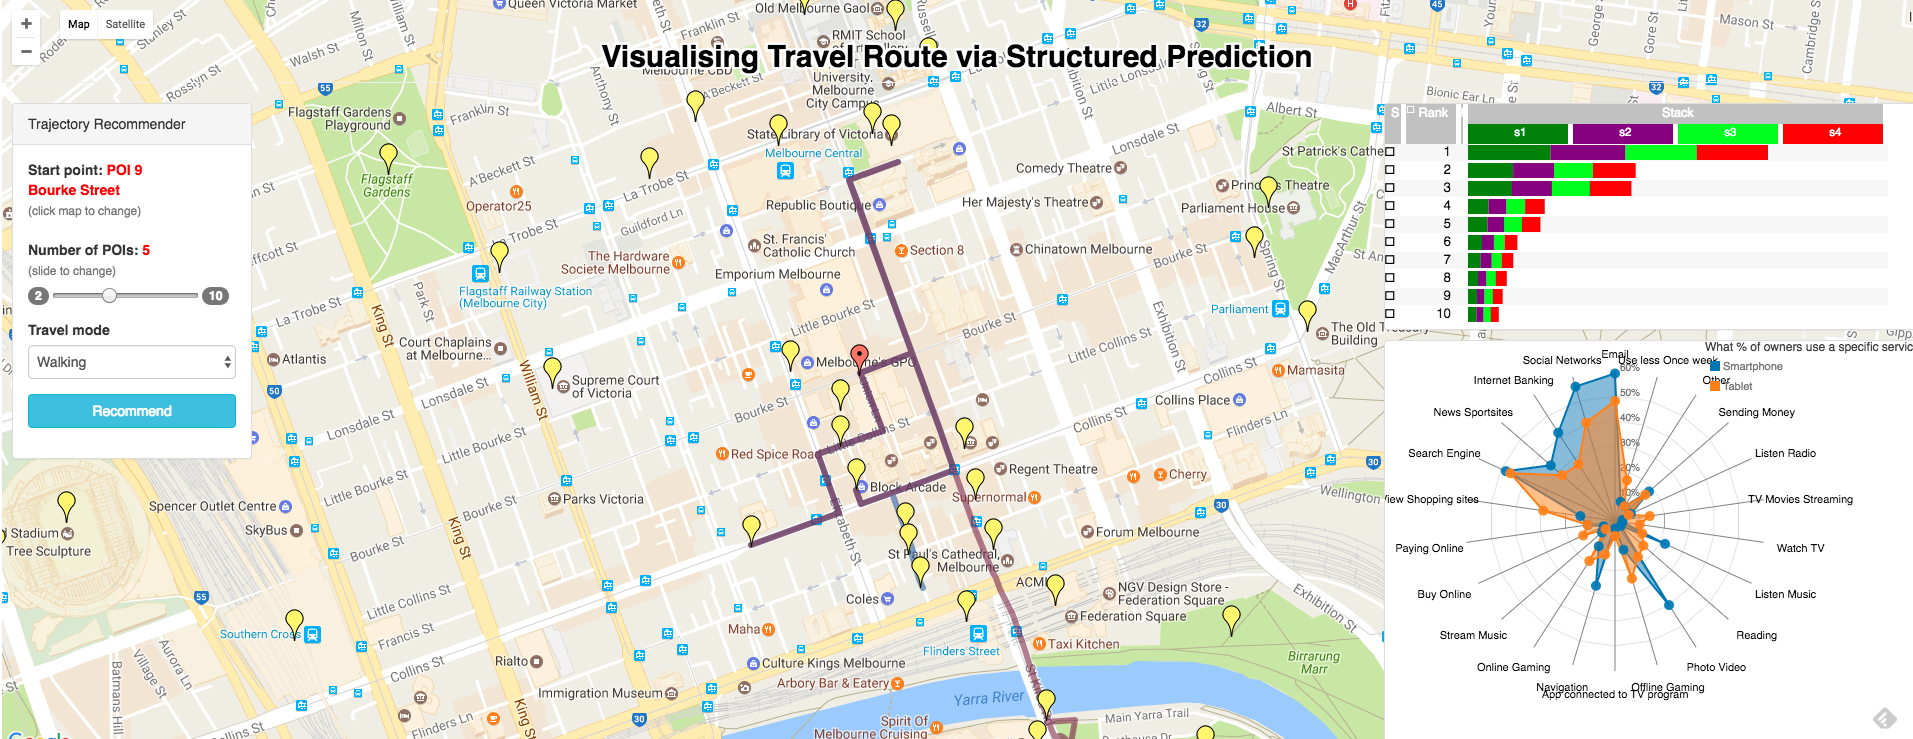
\includegraphics[width=0.9\textwidth]{figure/sample_map.png}
   \caption{Travel route visualisation system. Given a starting POI and a number of POI to be visited, the system recommends a set of routes from a history of previous tourists.}
   \label{fig:overview}
 \end{teaserfigure}

\maketitle


\section{Introduction}
%background
Sequence ranking has emerged as an important tool for solving diverse problems such as travel route and music playlist recommendations. Unlike the classical ranking algorithm where each item considers independently, the sequence ranking algorithm requires modelling a structure between items and suggests a set of items as a whole. For example, let us consider recommending a trajectory of points of interest (POI) in a city to a visitor. If the classical ranking algorithm learns a user's preference for each individual location while ignores the distances between them, the algorithm may create a long trajectory, which should be shorter in optimal routeing. Several sequence ranking algorithms are proposed to solve the problem and achieve relative success to compare with the classical algorithms. An important challenge remaining is to construct a visualisation of the recommendation system so that a user can analyse the suggested sequences and plan a better trip based on the interaction with the system.

%approach
In this paper, we tackle the problem of sequence visualisation, especially, in the travel route recommendation. We first define a travel route as a sequence of POIs and then formulate the sequence ranking algorithm as a structured prediction problem. Based on hand-crafted features for each POI and pairs of POIs, we train the prediction model with trajectory data extracted from geo-tagged photos. To visualise the suggested routes, we develop a novel tool that efficiently displays multiple suggested routes and helps users understand the process behind the recommendations. Specifically, our system decompose a total score of each route into a set of features and their corresponding scores and show the total score as a stacked bar plot of the features. The system also visualise differences between POIs in a single route to show how POIs in the single route can diverse to each other. This visualisation helps a tourist, who wants to have diverse experience, choose the best route among the set of recommended routes.

\section{Structured Prediction}
% don't need very details of the algorithm
% need problem definition
% copied from nips paper
Travel route recommendation problems involve a set of POIs in a city. Given a trajectory query $\mathbf{x} = (s, l)$, comprising a start POI $s$ and trip length $l$, i.e. the number of POIs to be visited during the trip including $s$, the goal is to suggest one or more sequences of POIs that maximise some notion of utility.

We first cast the travel recommendation as a structured prediction problem, which allows us to leverage the well-studied literature of structured SVMs (SSVM)~\cite{tsochantaridis2005large,joachims2009predicting}. There are two obstacles to prevent us applying the SSVM directly to the sequence recommendation problem; first, there would be multiple possible routes among a set of POIs, second, a naive application of SSVM would generate repeating sequence in the prediction time. 
To eliminate possible loop in a prediction time, we adopt serial list Viterbi~\cite{seshadri1994list,nill1995list} algorithm.
We finally trained our model on the trajectory data extracted from Flickr photos taken in Melbourne~\cite{chen2016learning}.

From a visualisation perspective, an important advantage of the SSVM is the explicit representation of feature score in its final decision process. Especially, in our case, we can disassemble the final score of a route into feature scores of each POI and each transition between two adjacency POIs. We hand-crafted POI features such as the category, popularity, average visit duration of previous tourists, etc, and also crafted transition features such as the distance and neighbourhood of two POIs.

\begin{figure}[t!]
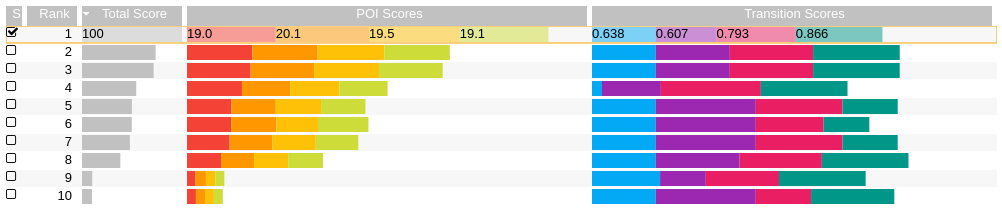
\includegraphics[width=0.9\linewidth]{figure/sample_stack.png}
\caption{Visualisation of feature scores for top ten recommended routes. ?What are the features here?}
\label{fig:stack}
\end{figure}

\section{Visualisation}
%what are the features we want to emphasis?
%make a bullet list of something like that
Our goal is to design an interactive visualisation system on top of the structured prediction framework.
Figure \ref{fig:overview} show the overview of live demo system, which consists of four major component: a map to display suggested routes, an input box for user query on the left side, a stacked score of routes on the upper right side, a radar chart to compare multiple features of POIs on lower right side. The role and construction of three major component are as follow:
\begin{itemize}
\item \textbf{User query} A query consists of a starting POI and a trip length. Users can choose the starting POI on the map and adjust slide to set the trip length. In addition, we support three different traveling modes: bicycling, walking, and driving. Based on the different mode, we optimise suggested routes between POIs in a sequence.
\item \textbf{Route score visualisation} A score of each route consists of different contributions of multiple attributes. While the visualisation of a proposed route is straightforward, its interpretation is not, because the rank of the route consists of multiple attributes. We adopt the LineUp framework~\cite{gratzl2013lineup} devised to support the visualisation of multi-attribute ranking via stacked representation. Figure \ref{fig:stack} shows the stacked scores of top ten recommended routes.
\item \textbf{POI feature visualisation} We further provide a tool to analyse a variation between multiple POIs in a single route. For example, Figure \ref{fig:radar} shows the feature scores of two POIs. 
\end{itemize}

\begin{figure}[t!]
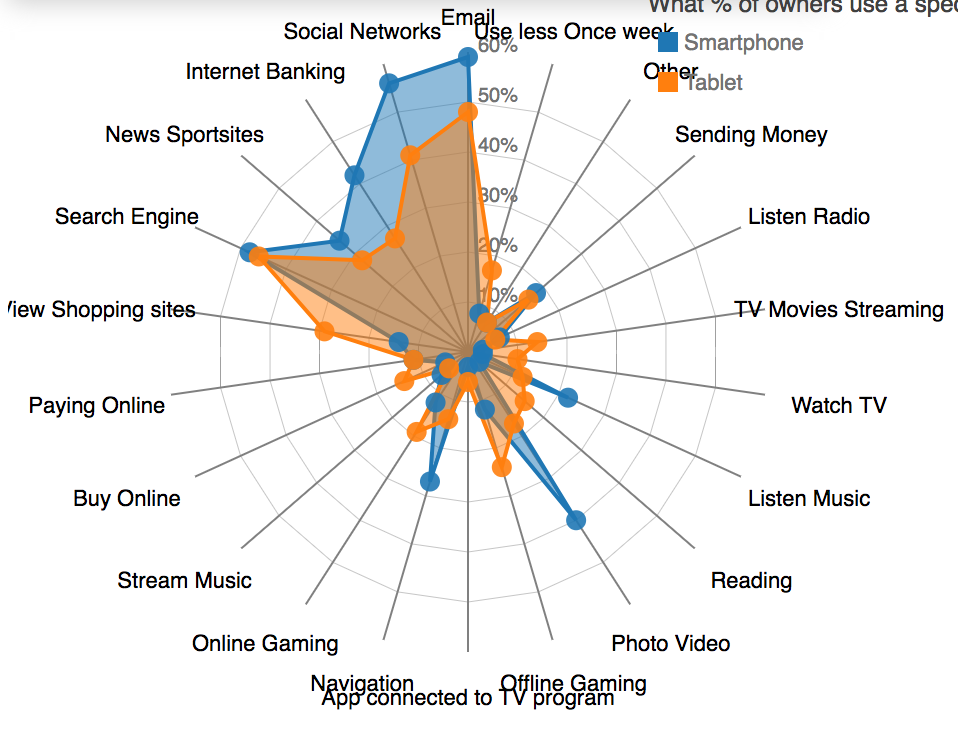
\includegraphics[width=0.8\linewidth]{figure/sample_radar.png}
\caption{Comparison between two POIs with respect to multiple features. We compare the Queen Victoria Market and Melbourne Aquarium. The Queen Victoria Market has a high score on \textit{shopping} and \textit{city precincts} features whereas the Melbourne aquarium has a high score on \textit{Entertainment} feature.}
\label{fig:radar}
\end{figure}


\section{Conclusion}
%summary
In this demonstration, we showcase an interactive route analyser which helps an interaction between users and route recommendation systems. The system benefits the explicit feature construction of the structured prediction model, and visualise recommended routes as well as relevant information on both route level and POI level.

\bibliographystyle{ACM-Reference-Format}
\bibliography{sigproc} 

\end{document}
